%!Tex Root = ../Main.tex
% ./Packete_und_Deklarationen.tex
\chapter{Einführung}
\label{ch:einführung}

\section{Compiler und Interpreter}
Der wohl wichtigsten zu klärenden Begriffe, sind die eines \colorbold{Compilers} (Definition~\ref{def:compiler}) und eines  \colorbold{Interpreters} (Definition~\ref{def:interpreter}), da das Schreiben eines Compilers von der \colorbold{PicoC-Sprache} in die \colorbold{RETI-Sprache} das Thema dieser Bachelorarbeit ist und die Definition eines \colorbold{Interpreters} genutzt wird, um zu definieren was ein \colorbold{Compiler} ist. Des Weiteren wurde zur \colorbold{Qualitätsicherung} ein \colorbold{RETI-Interpreter} implementiert, um mithilfe des \colorbold{GCC}\footnote{Sammlung von Compilern für Linux bzw. GNU-Linux, steht für \colorbold{G}NU \colorbold{C}ompiler \colorbold{C}ollection} und von \colorbold{Tests} die \colorbold{Beziehungen} in \ref{eq:compiler_beziehungen} zu belegen (siehe Subkapitel~\ref{sec:qualitätssicherung}).

\begin{Definition}{Interpreter}{interpreter}
  \colorbold{Interpretiert} die \colorbold{Instructions} bzw. \colorbold{Statements} eines Programmes $P$ direkt.

  Auf die Implementierung bezogen arbeitet ein Interpreter auf den compilerinternen \colorbold{Sub-Bäumen} des \colorbold{Abstract Syntax Tree} (Definition~\ref{def:abstrakte_syntax_tree}) und führt je nach Komposition der \colorbold{Nodes} des Abstract Syntax Tree, auf die er während des Darüber-Iterierens stösst unterschiedliche Anweisungen aus.
\end{Definition}

% https://tex.stackexchange.com/questions/51228/how-to-increase-the-horizontal-distance-between-nodes
\begin{Definition}{Compiler}{compiler}
  \colorbold{Kompiliert} ein Program $P_1$, welches in einer Sprache $L_1$ geschrieben ist, in ein Program $P_2$, welches in einer Sprache $L_2$ geschrieben ist.

  Wobei \colorbold{Kompilieren} meint, dass das Program $P_1$ in das Program $P_2$ übersetzt und bei beiden Programmen, wenn sie von \colorbold{Interpreter} ihrer jeweiligen Sprachen $L_1$ und $L_2$ \colorbold{interpretiert} werden, der gleiche \colorbold{Output} rauskommt. Also beide Programme $P_1$ und $P_2$ die gleiche \colorbold{Semantik} haben und sich nur \colorbold{syntaktisch} durch die Sprachen $L_1$ und $L_2$, in denen sie geschrieben stehen unterscheiden.

  \begin{equation}
    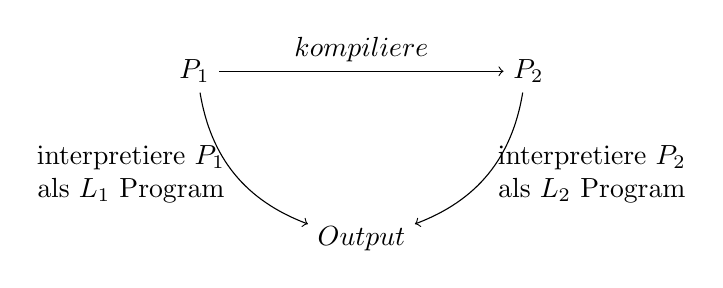
\begin{tikzpicture}[auto, baseline=(current  bounding  box.center)]
      \node (program1) at (135:3) {$P_{1}$};
      \node (program2) at (45:3) {$P_{2}$};
      \node (output)  at (270:0) {$Output$};

      % https://tex.stackexchange.com/questions/24372/how-to-add-newline-within-node-using-tikz
      \draw[->] (program1) to node[above] {$kompiliere$} (program2);
      \draw[->] (program1) to[bend right] node[left, align=center] {interpretiere $P_{1}$\\ als $L_{1}$ Program} (output);
      \draw[->] (program2) to[bend left] node[right, align=center] {interpretiere $P_{2}$\\ als $L_{2}$ Program} (output);
    \end{tikzpicture}
    \label{eq:compiler_beziehungen}
  \end{equation}
\end{Definition}

Üblicherweise kompiliert ein \colorbold{Compiler} von einer \colorbold{komplexeren Sprache} zu \colorbold{Maschinensprache}, aber es gibt z.B. auch \colorbold{Transpiler} (Definition~\ref{def:transpiler}) oder \colorbold{Cross-Compiler} (Definition~\ref{def:cross_compiler}).

% TODO vielleicht noch die Sache mit den 2 Bedeutungen von Assembler
% TODO: die Sache mit Blocks und GOTO in x_86, aber ehe später

\begin{Definition}{Transpiler (bzw. Source-to-source Compiler)}{transpiler}
  Kompiliert zwischen Sprachen, die ungefähr auf dem \colorbold{gleichen} Level an \colorbold{Abstraktion} arbeiten\footnote{Die im aktuellen Zeitgeist in Mode gekommene Sprache \colorbold{TypeScript} will als Obermenge von JavaScript und wird daher zu \colorbold{JavaScript} transpiliert.}.
  % TODO:
\end{Definition}

\begin{Definition}{Cross-Compiler}{cross_compiler}
  Kompiliert ein Program für eine Sprache, die auf der eigenen Maschine garnicht läuft.
\end{Definition}

  Ein \colorbold{Cross-Compiler} ist entweder notwendig, wenn noch kein oder niemals ein Compiler für die Wunschsprache existiert, der unter der \colorbold{Maschienensprache} $L_2$ einer Zielmaschine $M_2$ läuft oder die Zielmaschine $M_2$ nicht ausreichend \colorbold{Rechenleistung} hat, um ein Programm in der Wunschsprache zeitnah selbst zu kompilieren.
  \footnote{Lego Mindstorms} % TODO:

  Hat die Zielmaschine $M_2$ allerdings ausreichend Leistung, um Programme selbst zu kompilieren und es fehlt lediglich ein Compiler, der das übernimmt, so ist eine mögliche Lösung in einem ersten einen \colorbold{minimalen Compiler} zu schreiben, der die \colorbold{Wunschsprache} in die \colorbold{Maschienensprache} der Zielmaschine $M_2$ kompiliert. Diesen \colorbold{minimalen Compiler} könnte man nun komplett in der Maschinensprache


  und sich dafür die \colorbold{Rechenleistung} einer anderen Maschine borgt und eine beliebige \colorbold{Sprache}, die auf dieser Maschien läuft, in der dieser Minimale Compiler geschrieben wird.

  Hat man diesen \colorbold{minimalen Compiler} kann man Programme in der Wunschsprache schreiben und mithilfe des  \colorbold{minimalen Compilers} kompilieren, sodass diese Programme auf der Zielmaschine laufen.

  Nun kann man den \colorbold{minimalen Compiler}, denn man gerade eben in einer \colorbold{Programmesprache} implementiert hat, in der \colorbold{Wunschsprache} selbst implementieren und dann mit dem \colorbold{minamlen Compiler} für ebendiese Wunschsprache selbst kompilieren. Was man als Output bekommt ist ein \colorbold{minimmaler Compiler}, der aber auf der \colorbold{Zielmaschine} läuft und die \colorbold{Wunschsprache} in die \colorbold{Maschienensprache} der Zielmaschine kompiliert.

  Aufbauend auf diesem \colorbold{minimalen Compiler}, der auf der \colorbold{Zielmaschine} läuft, kann man nun auf der Zielmaschine selbst \colorbold{iterativ} den minimalen Compiler schrittweise zu einem umfangreicheren Compiler, der mehr Funktionalitäten unterstützt weiterentwickeln und braucht die ursprüngliche Maschine, auf dem man die allererste Version des minimalen Compilers implementiert hat nicht mehr. Dieses Vorgehen wird auch als \colorbold{Bootstrapping} (Definition~\ref{def:bootstrapping}) bezeichnet.\footnote{Der Begriff hat seinen Ursprung in der englischen Redewendung \glqq pulling yourself up by your own bootstraps\grqq, was im deutschen ungefähr der aus den Lügengeschichten des Freiherrn von Münchhausen bekannten Redewendung \glqq sich am eigenen Schopf aus dem Sumpf ziehen\grqq entspricht.}

  % Der Begriff ist sinnverwandt mit dem \colorbold{Booten} eines Computers, wo die wichtigste Software, der \colorbold{Kernel} zuerst in den Speicher geladen wird und darauf aufbauend von diesem dann das Betriebssysteme, welches bei Bedarf dann \colorbold{Systemsoftware}\footnote{Software, die das Ausführen von Anwendungssoftware ermöglicht oder unterstützt, wie z.B. Treiber.} und \colorbold{Anwendungssoftware}\footnote{Software, deren Anwendung darin besteht, dass sie dem Benutzer unmittelbar eine Dienstleistung zur Verfügung stellt.} lädt.

% Das ist das, was der PicoC-Compiler ist

\begin{Definition}{Bootstrapping}{bootstrapping}
  Es gibt zwei verschiedene Formen von \colorbold{Bootstrapping}:

  % https://www.overleaf.com/learn/latex/Counters
  \counterwithin{subdefcounter}{\tcbcounter}
  \setcounter{subdefcounter}{1}

  % https://tex.stackexchange.com/questions/7627/how-to-reference-paragraph
  \titleformat{\paragraph}[runin]{\normalfont\normalsize\bfseries}{}{0mm}{}[:]

  % https://tex.stackexchange.com/questions/7627/how-to-reference-paragraph
  \paragraph{\thesubdefcounter}\label{par:bootstrapping1}\hspace{-0.25cm}
  Wenn man ein \colorbold{Programm}, dass auf einer \colorbold{Maschine} $M_1$ läuft, auch auf einer \colorbold{Zielmaschine} $M_2$ zum laufen bringt.

  \stepcounter{subdefcounter}

  \paragraph{\thesubdefcounter}\label{par:bootstrapping2}\hspace{-0.25cm}
  Wenn man einen Compiler mithilfe von \colorbold{früheren Versionen} seiner selbst schreibt. Man schreibt den erweiterten Compiler in der Sprache, welche von der früheren Version des Compilers kompiliert wird und schafft es so iterativ immer umfangreichere Compiler zu bauen.\footcite{earley_formalism_1970}

\end{Definition}

Die Form von Bootstrapping in \nameref{par:bootstrapping1} bildet im Falle dessen, dass es sich beim dem Programm um einen Compiler für eine Programmiersprache handelt die Lösung für ein Problem, dass auf das \colorbold{Henne-Ei-Problem}\footnote{Beschreibt die Situation, wenn ein System sich selbst als Abhängigkeit hat, damit es überhaupt einen Anfang für dieses System geben kann. Dafür steht das Problem mit der Henne und dem Ei sinnbildlich, da hier die Frage ist, wie das ganze seinen Anfang genommen hat, da beides zirkular voneinander abhängt.} reduziert werden kann.

  Wenn es auf der Zielmaschine $M_2$ noch gar keinen Compiler für die Programmiersprache gibt, in der der Compiler für ebendiese Programmiersprache geschrieben steht, so liegt eine \colorbold{zirkulare Abhängigkeit vor}, die man nur auflösen kann, indem eine \colorbold{externe Entität} zur Hilfe nimmt.

  Eine Möglichkeit ist, indem man einen \colorbold{Cross-Compiler} auf der Maschine $M_1$ nutzt, der den \colorbold{Compiler} der Programmiersprache für die andere Maschine $M_2$ kompiliert bzw. \colorbold{bootstraped}.


\subsection{T-Diagramme}
\begin{Definition}{T-Diagram}{t_diagram}
\end{Definition}
% TODO: Darstelunng von Interpreter, Compiler und Cross-Compiler als T-Diagram.
% TODO: mehrere T's entsprehcen einem Comipler, Compilieren und dann Intepretieren entspricht einem großen Interpreter.
% TODO: Quelle nennen
\section{Grammatiken}
\section{Grundlagen}
\begin{Definition}{Sprache}{Sprache}
\end{Definition}
\begin{Definition}{Chromsky Hierarchie}{chromsky_hierarchie}
\end{Definition}
\begin{Definition}{Grammatik}{grammatik}
\end{Definition}
\begin{Definition}{Reguläre Sprachen}{reguläre_sprachen}
\end{Definition}
\begin{Definition}{Ableitung}{ableitung}
\end{Definition}
\begin{Definition}{Links- und Rechtsableitung}{links_und_rechtsableitung}
\end{Definition}
\begin{Definition}{Linksrekursive Grammatiken}{linksrekursive_grammatiken}
Eine \colorbold{Grammatik} ist \colorbold{linksrekursiv}, wenn sie ein  \colorbold{Nicht-Terminalsymbol} enthält, dass \colorbold{linksrekursiv} ist.

Ein \colorbold{Nicht-Terminalsymbol} ist  \colorbold{linksrekursiv}, wenn das \colorbold{linkeste Symbol} in einer seiner \colorbold{Produktionen} es selbst ist oder zu sich selbst gemacht werden kann durch eine Folge von Ableitungen:
\begin{equation*}
  A \Rightarrow^{*} Aa,
\end{equation*}
wobei $a$ eine beliebige Folge von \colorbold{Terminalsymbolen} und \colorbold{Nicht-Terminalsymbolen} ist.
\end{Definition}
\subsection{Mehrdeutige Grammatiken}
\begin{Definition}{Ableitungsbaum}{ableitungsbaum}
% TODO: Bild hierfür
\end{Definition}
\begin{Definition}{Mehrdeutige Grammatik}{mehrdeutige_grammatik}
% TODO: (Bild hierfür)
\end{Definition}
\subsection{Präzidenz und Assoziativität}
\begin{Definition}{Assoziativität}{assoziativität}
\end{Definition}
\begin{Definition}{Präzidenz}{präzidenz}
\end{Definition}
\begin{Definition}{Wortproblem}{wortproblem}
  % zu Grammatiken schieben
\end{Definition}
\begin{Definition}{LL(k)-Grammatik}{llk_grammatik}
  Eine Grammatik ist \colorbold{LL(k)} für $k\in\mathbb{N}$, falls jeder Ableitungsschritt eindeutig durch die nächsten $k$ \colorbold{Symbole} des \colorbold{Eingabeworts} bzw. in Bezug zu Compilerbau \colorbold{Token} des \colorbold{Inputstrings} zu bestimmen ist\footnote{Das wird auch als \colorbold{Lookahead} von $k$ bezeichnet.}. Dabei steht \colorbold{LL} für \colorbold{l}eft-to-right und \colorbold{l}eftmost-derivation, da das \colorbold{Eingabewort} von \colorbold{links nach rechts} geparsed und immer \colorbold{Linksableitungen} genommen werden müssen\footnote{Wobei sich das mit den \colorbold{Linksableitungen} automatisch ergibt, wenn man das Eingabewort von  \colorbold{links-nach-rechts} parsed und jeder der nächsten $k$ \colorbold{Ableitungsschritte} eindeutig sein soll.}, damit die obige Bedingung mit den \colorbold{nächsten} $k$ Symbolen gilt.
\end{Definition}
\begin{Definition}{Kontextfreie Sprachen}{kontextfreie_sprachen}
\end{Definition}
% \subsection{Linksrekursiv und Rechtrekursiv}
\section{Lexikalische Analyse}
\label{sec:lexikalische_analyse}

Die \colorbold{Lexikalische Analyse} bildet üblicherweise die erste Ebene innerhalb der \colorbold{Pipe Architektur} bei der Implementierung von Compilern. Die Aufgabe der lexikalischen Analyse ist vereinfacht gesagt, in einem Inputstring, z.B. dem Inhalt einer Datei, welche in \colorbold{UTF-8} codiert ist, Folgen endlicher Symbole (auch \colorbold{Wörter} genannt) zu finden, die bestimmte \colorbold{Pattern} (Definition~\ref{def:pattern}) matchen, die durch eine \colorbold{reguläre Grammatik} spezifiziert sind.

\begin{Definition}{Pattern}{pattern}
  \colorbold{Beschreibung} aller möglichen \colorbold{Lexeme} einer Menge $\mathbb{P}_{T}$, die einem bestimmten \colorbold{Token} $T$ zugeordnet werden.
  Die Menge $\mathbb{P}_{T}$ ist eine möglicherweise unendliche Menge von \colorbold{Wörtern}, die sich mit den Produktionen einer \colorbold{regulären Grammatik} ${G}_{Lex}$ einer \colorbold{regulären Sprache} ${L}_{Lex}$ beschreiben lassen \footnote{Als Beschreibungswerkzeug können aber auch z.B. reguläre Ausdrücke hergenommen werden.}, die für die Beschreibung eines \colorbold{Tokens} $T$ zuständig sind.\footcite{noauthor_what_nodate}
\end{Definition}

Diese Folgen endlicher Symoble werden auch \colorbold{Lexeme} (Definition~\ref{def:lexeme}) genannt.

\begin{Definition}{Lexeme}{lexeme}
  Ein \colorbold{Lexeme} ist ein \colorbold{Wort} aus dem Inputstring, welches das \colorbold{Pattern} für eines der \colorbold{Token} $T$ einer \colorbold{Sprache} ${L}_{Lex}$ matched.
\footcite{noauthor_what_nodate}
\end{Definition}

Diese \colorbold{Lexeme} werden vom \colorbold{Lexer} im \colorbold{Inputstring} identifziert und \colorbold{Tokens} $T$ zugeordnet (Definition~\ref{def:lexer}). Die \colorbold{Tokens} sind es, die letztendlich an die \colorbold{Syntaktische Analyse} weitergegeben werden.

\begin{Definition}{Lexer (bzw. Scanner)}{lexer}
  Ein \colorbold{Lexer} ist eine \colorbold{partielle} Funktion \hspace{0.2cm}$lex: \Sigma^{*} \rightharpoonup (N \times W)^{*}$, welche ein \colorbold{Wort} aus $\Sigma^{*}$ auf ein \colorbold{Token} $T$ mit einem \colorbold{Tokennamen} $N$ und einem \colorbold{Tokenwert} $W$ abbildet, falls diese Folge von Symbolen sich unter der \colorbold{regulären Grammatik} ${G}_{Lex}$, der \colorbold{regulären Sprache} ${L_{Lex}}$ abbleiten lässt.\footcite{noauthor_lecture-notes-2021_2022}
\end{Definition}

Ein \colorbold{Lexer} ist im Allgemeinen eine \colorbold{partielle Funktion}, da es Zeichenfolgen geben kann, die kein \colorbold{Pattern} eines \colorbold{Tokens} der Sprache $L_{Lex}$ matchen. In Bezug auf eine Implementierung, wird, wenn der Lexer Teil der Implementierung eines Compilers ist, in diesem Fall eine \colorbold{Fehlermeldung} ausgegeben.

Eine weitere Aufgabe der \colorbold{Lekikalischen Analyse} ist es jegliche für die Weiterverarbeitung unwichtigen Symbole, wie Leerzeichen \,\textvisiblespace\,, Newline \verb|\n|\footnote{In Unix Systemen wird für Newline das ASCII Symbol \colorbold{line feed}, in Windows hingegen die ASCII Symbole \colorbold{carriage return} und \colorbold{line feed} nacheinander verwendet. Das wird aber meist durch die verwendete Porgrammiersprache, die man zur Inplementierung des Lexers nutzt wegabstrahiert.} und Tabs \verb|\t| aus dem Inputstring herauszufiltern. Das geschieht mittels des \colorbold{Lexers}, der allen für die \colorbold{Syntaktische Analyse} unwichtige Zeichen das leere Wort $\epsilon$ zuordnet. Das ist auch im Sinne der Definition, denn $\epsilon \in \Sigma^{*}$.
Nur das, was für die \colorbold{Syntaktische Analyse} wichtig ist, soll weiterverarbeitet werden, alles andere wird herausgefiltert.

Der Grund warum nicht einfach nur die \colorbold{Lexeme} an die \colorbold{Syntaktische Analyse} weitergegeben werden und der Grund für die Aufteilung des \colorbold{Tokens} in \colorbold{Tokenname} und \colorbold{Tokenwert} ist, weil z.B. die Bezeichner von Variablen, Konstanten und Funktionen beliebige Zeichenfolgen sein können, wie \smalltt{my\_fun}, \smalltt{my\_var} oder \smalltt{my\_const} und es auch viele verschiedenen Zahlen gibt, wie \smalltt{42}, \smalltt{314} oder \smalltt{12}. Die Überbegriffe bzw. Tokennamen für beliebige Bezeichner von Variablen, Konstanten und Funktionen und beliebige Zahlen sind aber trotz allem z.B. \smalltt{Zahl} und \smalltt{Bezeichner}.

Ein \colorbold{Lexeme} ist damit aber nicht das gleiche, wie der \colorbold{Tokenwert}, denn z.B. im Falle von PicoC kann z.B. der Wert $99$ durch zwei verschiedene Literale darstellt werden, einmal als ASCII-Zeichen \smalltt{'c'} und des Weiteren auch in Dezimalschreibweise als \smalltt{99}\footnote{Die Programmiersprache Python erlaubt es z.B. diesern Wert auch mit den Literalen \smalltt{0b1100011} und \smalltt{0x63} darzustellen.}. Der \colorbold{Tokenwert} ist jedoch der letztendliche Wert an sich, unabhängig von der Darstellungsform.

  Die \colorbold{Grammatik} $G_{Lex}$, die zur Beschreibung der Token $T$ einer regulären Sprache $L_{Lex}$ verwendet wird, ist üblicherweise \colorbold{regulär}, da ein typischer \colorbold{Lexer} immer nur \colorbold{ein Symbol} vorausschaut\footnote{Man nennt das auch einem \colorbold{Lookahead} von $1$}, unabhängig davon, was für Symbole davor aufgetaucht sind. Die übliche Implementierung eines \colorbold{Lexers} merkt sich nicht, was für Symbole davor aufgetaucht sind.

% TODO: später erwähnen, dass alle Produtkionen der Grammatik G_lex eine reguläre Form haben, was der Beweis ist

\begin{Special_Paragraph}
  Um Verwirrung verzubäugen ist es wichtig folgende Unterscheidung hervorzuheben: Wenn von \colorbold{Symbolen} die Rede ist, so werden in der \colorbold{Lexikalischen Analyse}, der \colorbold{Syntaktische Analyse} und der \colorbold{Code Generierung}, auf diesen verschiedenen Ebenen unterschiedliche Konzepte als Symbole bezeichnet.

  In der Lexikalischen Analyse sind einzelne \colorbold{Zeichen eines Zeichensatzes} die Symbole.

  In der Syntaktischen Analyse sind die \colorbold{Tokennamen} die Symbole.

  In der Code Generierung sind die \colorbold{Bezeichner von Variablen, Konstanten und Funktionnen} die Symbole\footnote{Das ist der Grund, warum die Tabelle, in der Informationen zu Identifiern gespeichert werden aus Kapitel~\ref{ch:implementierung} Symboltabelle genannt wird.}.
\end{Special_Paragraph}

\begin{Definition}{Literal}{literal}
  Eine von möglicherweise vielen weiteren \colorbold{Darstellungsformen} für ein und denselben \colorbold{Wert}.
  % TODO: vielleicht schönes Bildchen
\end{Definition}

Um eine Gesamtübersicht über die \colorbold{Lexikalische Analyse} zu geben, ist in Abbildung~\ref{fig:lexikalische_analyse_veranschaulichung} die Lexikalische Analyse an einem Beispiel veranschaulicht.

\begin{figure}[H]
  \codebox[title=Inputstring, remember as=inputstring, width=0.2\linewidth, nobeforeafter]{./code_examples/example1.picoc}
  \hfill
  \treebox[title=Tokenfolge, remember as=tokenfolge, width=0.6\linewidth, nobeforeafter]{./code_examples/example1.tokens}

  \begin{tikzpicture}[overlay,remember picture,line width=1mm,draw=PrimaryColor]
  \draw[->] (inputstring.east) to[bend right] node[above] {Lexer} (tokenfolge.west);
  \end{tikzpicture}
  \caption{Veranschaulichung der Lexikalischen Analyse}
  \label{fig:lexikalische_analyse_veranschaulichung}
\end{figure}

\section{Syntaktische Analyse}
In der \colorbold{Syntaktischen Analyse} ist für einige Sprachen eine \colorbold{Kontextfreie Grammatik} $G_{Parse}$ notwendig, um diese Sprache zu beschreiben, da viele Programmiersprachen z.B. für \colorbold{Funktionsaufrufe} \verb|fun(arg)| und \colorbold{Codeblöcke} \verb|if(1){}| syntaktische Mittel verwenden, die es notwendig machen sich zu merken wieviele öffnende Klammern \verb|'('| bzw. öffnende geschweifte Klammern \verb|'{'| es momentan gibt, die noch nicht durch eine enstsprechende schließende Klammer \verb|')'| bzw. schließende geschweifte Klammer \verb|'}'| geschlossen wurden.

% TODO: später erwähnen, dass alle Produktionen der Grammatik G_parse eine kontexfreie Form haben, was der Beweis ist

Die \colorbold{Syntax}, in welcher der \colorbold{Inputstring} aufgeschrieben ist, wird auch als \colorbold{Konkrette Syntax} (Definition~\ref{def:konkrette_syntax}) bezeichnet. In einem Zwischenschritt, dem \colorbold{Parsen} wird aus diesem Inputstring mithilfe eines \colorbold{Parsers} (Definition~\ref{def:parser}), ein \colorbold{Derivation Tree} (Definition~\ref{def:derivation_tree}) generiert, der als Zwischenstufe hin zum einem \colorbold{Abstrakt Syntax Tree} (Definition~\ref{def:abstrakte_syntax_tree}) dient. Für einen ordentlichen Code ist es vor allem im Compilerbau förderlich kleinschrittig vorzugehen, deshalb erst die Generierung des \colorbold{Derivation Tree} und dann der \colorbold{Abstrakt Syntax Tree}.

\begin{Definition}{Konkrette Syntax}{konkrette_syntax}
  \colorbold{Syntax} einer \colorbold{Sprache}, die durch die \colorbold{Grammatiken} $G_{Lex}$ und $G_{Parse}$ zusammengenommen beschrieben wird.

  Ein \colorbold{Programm} in seiner \colorbold{Textrepräsentation}, wie es in einer Textdatei nach den Produktionen der \colorbold{Grammatiken} $G_{Lex}$ und $G_{Parse}$ abgeleitet steht, bevor man es kompiliert, ist in \colorbold{Konkretter Syntax} aufgeschrieben.\footcite{noauthor_course_2022}
\end{Definition}

\begin{Definition}{Derivation Tree (bzw. Parse Tree)}{derivation_tree}
  \colorbold{Compilerinterne Darstellung} eines in \colorbold{Konkretter Syntax} geschriebenen Inputstrings als \colorbold{Baumdatenstruktur}, in der \colorbold{Nichtterminalsymbole} die \colorbold{Inneren Knoten} des Baumes und \colorbold{Terminalsymbole} die \colorbold{Blätter} des Baumes bilden. Jede \colorbold{Produktions} der \colorbold{Grammatik} $G_{Parse}$, die ein Teil der \colorbold{Konkrette Syntax} ist,  wird zu einem eigenen \colorbold{Knoten}.

  Der \colorbold{Derivation Tree} wird optimalerweise immer so konstruiert bzw. die \colorbold{Konkrette Syntax} immer so definiert, dass sich möglichst einfach ein \colorbold{Abstrakt Syntax Tree} daraus konstruieren lässt.

% TODO: vielleicht ein hübsches Bildchen
\end{Definition}

\begin{Definition}{Parser}{parser}
  Ein Programm, dass eine \colorbold{Eingabe} in eine für die \colorbold{Weiterverbeitung} taugliche Form bringt.

  % https://www.overleaf.com/learn/latex/Counters
  \counterwithin{subdefcounter}{\tcbcounter}
  \setcounter{subdefcounter}{1}

  % https://tex.stackexchange.com/questions/7627/how-to-reference-paragraph
  \titleformat{\paragraph}[runin]{\normalfont\normalsize\bfseries}{}{0mm}{}[:]

  % https://tex.stackexchange.com/questions/7627/how-to-reference-paragraph
  \paragraph{\thesubdefcounter}\label{par:parser}\hspace{-0.25cm}
  In Bezug auf Compilerbau ist ein \colorbold{Parser} ein Programm, dass einen Inputstring von \colorbold{Konkretter Syntax} in die compilerinterne Darstellung eines \colorbold{Derivation Tree} übersetzt, was auch als  \colorbold{Parsen} bezeichnet wird\footnote{Es gibt allerdings auch alternative Definitionen, denen nach ein Parser in Bezug auf Compilerbau ein Programm ist, dass einen Inputstring von \colorbold{Konkretter Syntax} in  \colorbold{Abstrakte Syntax} übersetzt. Im Folgenden wird allerdings die obigte Definition \nameref{par:parser} verendet.}.\footcite{noauthor_compiler_nodate}
\end{Definition}

\begin{Special_Paragraph}
  An dieser Stelle könnte möglicherweise eine Begriffsverwirrung enstehen, ob ein \colorbold{Lexer} nach der obigen Definition nicht auch ein \colorbold{Parser} ist.

  In Bezug auf Compilerbau ist ein \colorbold{Lexer} ein Teil eines Parsers. Der Parser vereinigt sowohl die \colorbold{Lexikalische Analyse}, als auch einen Teil der \colorbold{Syntaktischen Analyse} in sich. Aber für sich isoliert, ohne Bezug zu Compilerbau betrachtet, ist ein Lexer nach Definition~\ref{def:parser} ebenfalls ein Parser. Aber im Compilerbau hat \colorbold{Parser} eine spezifischere Definition und hier überwiegt beim \colorbold{Lexer} seine Funktionalität, dass er den Inputstring lexikalisch weiterverarbeitet, um ihn als Lexer zu bezeichnen, der Teil eines Parsers ist.
\end{Special_Paragraph}

Die vom \colorbold{Lexer} im Inputstring identifizierten \colorbold{Token} werden in der \colorbold{Syntaktischen Analyse} vom \colorbold{Parser} (Definition~\ref{def:parser}) als \colorbold{Wegweiser} verwendet, da je nachdem, in welcher Reihenfolge die \colorbold{Token} auftauchen, dies einer anderen Ableitung in der \colorbold{Grammatik} $G_{Parse}$ entspricht. Dabei wird in der Grammatik nach dem \colorbold{Tokennamen} unterschieden und nicht nach dem Tokenwert, da es nur von Interesse ist, ob an einer bestimmten Stelle z.B. eine \verb|Zahl| steht und nicht, welchen konkretten Wert diese \verb|Zahl| hat. Der \colorbold{Tokenwert} ist erst später in der \colorbold{Code Generierung} in~\ref{sec:code_generierung} relevant.

Ein \colorbold{Parser} ist genauergesagt ein erweiterter \colorbold{Recognizer} (Definition~\ref{def:recognizer}), denn ein Parser löst das \colorbold{Wortproblem} (Definition~\ref{def:wortproblem}) für die \colorbold{Sprache}, die durch die \colorbold{Konkrette Syntax} beschrieben wird und konstruiert parallel dazu oder im Nachgang aus den Informationen, die während der Ausführung des Recognition Algorithmus gesichert wurden den \colorbold{Derivation Tree}.

\begin{Definition}{Recognizer (bzw. Erkenner)}{recognizer}
  Entspricht dem Maschinenmodell eines \colorbold{Automaten}. Im Bezug auf Compilerbau entspricht der \colorbold{Recognizer} einem \colorbold{Kellerautomaten}, in dem \colorbold{Wörter} bestimmter \colorbold{Kontextfreier Sprachen} erkannt werden. Der \colorbold{Recognizer} erkennt, ob ein Iputstring bzw. \colorbold{Wort} sich mit den Produktionen der \colorbold{Konkrette Syntax} ableiten lässt, also ob er bzw. es Teil der Sprache ist, die von der \colorbold{Konkretten Syntax} beschrieben wird oder nicht\footnote{Das vom \colorbold{Recognizer} gelöste Problem ist auch als \colorbold{Wortproblem} bekannt.}.
\end{Definition}

\begin{Special_Paragraph}
Für das \colorbold{Parsen} gibt es grundsätzlich \colorbold{zwei} verschiedene Ansätze:

% https://tex.stackexchange.com/questions/12373/how-to-change-the-space-between-the-itemize-items-in-latex
% https://stackoverflow.com/questions/1061112/eliminate-space-before-beginitemize
\begin{itemize}[itemsep=-1mm, topsep=-1mm]
  \coloritem[Top-Down Parsing] Der \colorbold{Derivation Tree} wird von \colorbold{oben-nach-unten} generiert, also von der \colorbold{Wurzel} zu den \colorbold{Blättern}. Dementsprechend fängt die Generierung des \colorbold{Derivation Tree} mit dem \colorbold{Startsymbol} der \colorbold{Grammatik} an und wendet in jedem Schritt eine \colorbold{Linksableitung} auf die \colorbold{Nicht-Terminalsymbole} an, bis man \colorbold{Terminalsymbole} hat und der gewünschte \colorbold{Inputstring} abgeleitet wurde oder es sich herausstellt, dass dieser nicht abgeleitet werden kann.\footcite{noauthor_what_nodate-2}

  Der Grund, warum die \colorbold{Linksableitung} verwendet wird und nicht z.B. die \colorbold{Rechtsableitung} ist, weil der das \colorbold{Eingabewert} bzw. der \colorbold{Inputstring} von \colorbold{links nach rechts} eingelesen wird, was gut damit zusammenpasst, dass die \colorbold{Linksableitung} die \colorbold{Blätter} von \colorbold{links-nach-rechts} generiert.

  Welche der \colorbold{Produktionen} für ein \colorbold{Nicht-Terminalsymbol} angewandt wird, wenn es mehrere Alternativen gibt, wird entweder durch \colorbold{Backtracking} oder durch \colorbold{Vorausschauen} gelöst.

  Eine sehr einfach zu implementierende Technik für \colorbold{Top-Down Parser} ist hierbei der \colorbold{Rekursive Abstieg}. Dabei wird jedem \colorbold{Nicht-Terminalsymbol} eine \colorbold{Prozedur} zugeordnet, welche die Produktionsregeln dieses \colorbold{Nicht-Terminalsymbols} umsetzt. Prozeduren rufen sich dabei wechselseitig gegenseitig entsprechend der \colorbold{Produktionsregeln} auf, falls eine entsprechende Produktionsregel eine \colorbold{Rekursion} enthält.

  \colorbold{Rekursiver Abstieg} kann mit \colorbold{Backtracking} verbunden werden, um auch Grammatiken parsen zu können, die nicht \colorbold{LL(k)} (Definition~\ref{def:llk_grammatik}) sind. Dabei werden meist nach dem \colorbold{Depth-First-Search Prinzip} alle \colorbold{Produktionen} für ein \colorbold{Nicht-Terminalsymbol} solange durchgegangen bis der gewüschte Inpustring abgeleitet ist oder alle \colorbold{Alternativen} für einen Schritt abgesucht sind, bis man wieder beim ersten Schritt angekommen ist und da auch alle \colorbold{Alternativen} abgesucht sind. Mit dieser Methode ist das Parsen \colorbold{Linksrekursiver Grammatiken} (Definition~\ref{def:linksrekursive_grammatiken}) allerdings nicht möglich, ohne die Grammatik vorher umgeformt zu haben und jegliche \colorbold{Linksrekursion} aus der \colorbold{Grammatik} entfernt zu haben, da diese zu \colorbold{Unendlicher Rekursion} führt\footnote{Diese Art von Parser wurde im \colorbold{PicoC-Compiler} implementiert, als dieser noch auf dem Stand des \colorbold{Bachelorprojektes} war, bevor er durch den nicht selbst implementierten \colorbold{Earley Parser} von \colorbold{Lark} (siehe \cite{noauthor_lark_2022}) ersetzt wurde.}

  Wenn man eine \colorbold{LL(k)} Grammatik hat, kann man auf \colorbold{Backtracking verzichten} und es reicht einfach nur immer $k$ \colorbold{Symbole} im \colorbold{Eingabewort} bzw. in Bezug auf Compilerbau \colorbold{Token} im \colorbold{Inpustring} vorauszuschauen. \colorbold{Mehrdeutige Grammatiken} sind dadurch ausgeschlossen, weil \colorbold{LL(k)} keine \colorbold{Mehrdeutigkeit} zulässt.\footnote{Diese Art von Parser ist im \colorbold{RETI-Interpreter} implementiert, da die \colorbold{RETI-Sprache} eine besonders simple \colorbold{LL(1) Grammatik} besitzt. Dieser \colorbold{Parser} wird auch als \colorbold{Predictive Parser} oder \colorbold{LL(k) Recursive Descent Parser} bezeichnet, wobei \colorbold{Recursive Descent} das englische Wort für \colorbold{Rekursiven Abstieg} ist.}
  \coloritem[Bottom-Up Parsing] Es wird mit dem \colorbold{Eingabewort} bzw. \colorbold{Inputstring} gestartet und versucht \colorbold{Rechtsableitungen}, entsprechend der \colorbold{Produktionen} der \colorbold{Konkretten Syntax} rückwärts anzuwenden bis man beim \colorbold{Startsymbol} landet.\footcite{noauthor_what_nodate-1}
  \coloritem[Chart Parser] Es wird \colorbold{Dynamische Programmierung} verwendet und partielle Zwischenergebnisse werden in einer \colorbold{Tabelle} (bzw. einem \colorbold{Chart}) gespeichert und können wiederverwendet werden. Das macht das Parsen \colorbold{Kontextfreier Grammatiken} effizienter, sodass es nur noch \colorbold{polynomielle} Zeit braucht, da \colorbold{Backtracking} nicht mehr notwendig ist.\footnote{Der \colorbold{Earley Parser}, den \colorbold{Lark} und damit der \colorbold{PicoC-Compiler} verwendet fällt unter diese Kategorie}
\end{itemize}
  % ein hübsches Bildchen, wo man einen Überblick bekommt
\end{Special_Paragraph}

% Problem mit Linksrekursion und Mehrdeutigkeit ansprechen

Der \colorbold{Abstrakt Syntax Tree} wird mithilfe von \colorbold{Transformern} (Definition~\ref{def:transformer}) und \colorbold{Visitors} (Definition~\ref{def:visitor}) generiert und ist das Endprodukt der \colorbold{Syntaktischen Analyse}. Wenn man die gesamte \colorbold{Syntaktische Analyse} betrachtet, so übersetzt diese einen Inpustring von der \colorbold{Konkretten Syntax} in die \colorbold{Abstrakte Syntax} (Definition~\ref{def:abstrakte_syntax}).

Die \colorbold{Baumdatenstruktur} des \colorbold{Derivation Tree} und  \colorbold{Abstrakt Syntax Tree} ermöglicht es die Operationen, die der Compiler bei der Weiterverarbeitung des Inputstrings ausführen muss möglichst \colorbold{effizient} auszuführen.

\begin{Definition}{Transformer}{transformer}
Ein Programm, dass von \colorbold{unten-nach-oben}, nach dem \colorbold{Breadth First Search} Prinzip alle Knoten des \colorbold{Derivation Tree} besucht und in Bezug zu Compilerbau, beim Antreffen eines bestimmten Knoten des \colorbold{Derivation Tree} einen entsprechenden Knoten des \colorbold{Abstrakt Syntax Tree} erzeugt und diesen anstelle des Knotens des \colorbold{Derivation Tree} setzt und so Stück für Stück den \colorbold{Abstrak Syntax Tree} konstruiert.
\end{Definition}

\begin{Definition}{Visitor}{visitor}
Ein Programm, dass von \colorbold{unten-nach-oben}, nach dem \colorbold{Breadth First Search} Prinzip alle Knoten des \colorbold{Derivation Tree} besucht und in Bezug zu Compilerbau, beim Antreffen eines bestimmten \colorbold{Knoten} des Derivation Tree, diesen \colorbold{in-place} mit anderen Knoten \colorbold{tauscht} oder \colorbold{manipuliert}, um den Derivation Tree für die weitere Verarbeitung durch z.B. einen Transformer zu vereinfachen.

Kann theoretisch auch zur Konstruktion eines \colorbold{Abstrakt Syntax Tree} verwendet werden, wenn z.B. eine externe Klasse verwendet wird, welches für die Konstruktion des \colorbold{Abstrakt Syntax Tree} verantwortlich ist, aber dafür ist ein \colorbold{Transformer} besser geeignet.
\end{Definition}

\begin{Definition}{Abstrakte Syntax}{abstrakte_syntax}
  \colorbold{Syntax}, die beschreibt, was für Arten von \colorbold{Komposition} bei den \colorbold{Knoten} eines \colorbold{Abstrakt Syntax Trees} möglich sind.\footcite{noauthor_course_2022}

  Jene Produktionen, die in der \colorbold{Konkretten Syntax} für die Umsetzung von \colorbold{Präzidenz} notwendig waren, sind in der \colorbold{Abstrakten Syntax} abgeflacht.
\end{Definition}

\begin{Definition}{Abstrakt Syntax Tree}{abstrakte_syntax_tree}
  \colorbold{Compilerinterne Darstellung} eines Programs, in welcher sich anhand der Knoten auf dem Pfad von der Wurzel zu einem \colorbold{Blatt} nicht mehr direkt nachvollziehen lässt, durch welche \colorbold{Produktionen} dieses Blatt abgeleitet wurde.

Der \colorbold{Abstrakt Syntax Tree} hat einmal den Zweck, dass die Kompositionen, die die Konten bilden können \colorbold{semantisch} näher an den \colorbold{Instructions eines Assemblers} dran sind und, dass man mit ihm bei der Betrachtung eines \colorbold{Knoten}, der für einen Teil des Programms steht, möglichst schnell die Frage beantworten kann, welche \colorbold{Funktionalität} der Sprache dieser umsetzt, welche \colorbold{Bestandteile} er hat und welche Funktionalität der Sprache diese Bestandteile umsetzen usw.\footcite{noauthor_course_2022}
\end{Definition}

Je weiter \colorbold{unten}\footnote{In der Informatik wachsen \colorbold{Bäume} von \colorbold{oben-nach-unten}. Die \colorbold{Wurzel} ist also \colorbold{oben}.} und \colorbold{links} ein Knoten im \colorbold{Abstrakt Syntax Tree} liegt, desto eher wird dieser Knoten komplett abgearbeitet sein, da in der \colorbold{Code Generierung} die Knoten nach dem \colorbold{Depth First Search} Prinzip abgearbeitet werden.

Um eine Gesamtübersicht über die \colorbold{Syntaktische Analyse} zu geben, ist in Abbildung~\ref{fig:syntaktische_analyse_veranschaulichung} die Syntaktische mit dem Beispiel aus Subkapitel~\ref{sec:lexikalische_analyse} fortgeführt.

\pagebreak
% https://tex.stackexchange.com/questions/8625/force-figure-placement-in-text
\begin{figure}[H]
  \centering
  \treebox[title=Tokenfolge, remember as=tokenfolge, width=0.6\linewidth, nobeforeafter]{./code_examples/example1.tokens}
  \hfill
  \treebox[title=Abstract Syntax Tree, remember as=abstract_sytax_tree, width=0.3\linewidth, nobeforeafter]{./code_examples/example1.ast}
  \vspace{2cm}
  \treebox[title=Derivation Tree, remember as=derivation_tree, width=0.6\linewidth]{./code_examples/example1.dt}

  \begin{tikzpicture}[overlay,remember picture,line width=1mm,draw=PrimaryColor]
    \draw[->] (tokenfolge.south) to node[left] {Parser} (derivation_tree.north);
    \draw[->] (derivation_tree.north) to node[right] {Visitors und Transformer} (abstract_sytax_tree.south);
  \end{tikzpicture}
  \caption{Veranschaulichung der Syntaktischen Analyse}
  \label{fig:syntaktische_analyse_veranschaulichung}
\end{figure}

\section{Code Generierung}
\label{sec:code_generierung}
\begin{Definition}{Pass}{pass}
% TODO: Bild semantisch gleiche Bedeutung
% TODO: auf T-Diagramme zurückkommen
\end{Definition}
\section{Fehlermeldungen}
\begin{Definition}{Fehlermeldung}{fehlermeldung}
\end{Definition}

% Kategorien von Fehlermeldungen
